% coding:utf-8

%kugprg, a LaTeX-Code for a summary of programming modules
%Copyright (C) 2013, Daniel Winz, Ervin Mazlagic

%This program is free software; you can redistribute it and/or
%modify it under the terms of the GNU General Public License
%as published by the Free Software Foundation; either version 2
%of the License, or (at your option) any later version.

%This program is distributed in the hope that it will be useful,
%but WITHOUT ANY WARRANTY; without even the implied warranty of
%MERCHANTABILITY or FITNESS FOR A PARTICULAR PURPOSE.  See the
%GNU General Public License for more details.
%----------------------------------------


\newpage
\subsection{Quicksearch}

Mit dem Quicksearch Algorithmus kann man ein Pattern in einer 
Zeichenfolge lokalisieren. Hierzu benötigt man einerseits das
Pattern \verb!p! und die Zeichenfolge \verb!a!.

\begin{table}[h!]
	\centering
	\begin{tabular}{l c l}
		Zeichenfolge
			& \verb!a!
			& \verb!ABADDBCCCABAACBB! \\
		Pattern
			& \verb!p!
			& \verb!ABAC! \\
	\end{tabular}
\end{table}

\noindent
Um das Pattern zu lokalisieren benötigt man ein Shiftarray \verb!s!.
Dieses muss speziell initialisert werden. Hierzu muss als erstes die 
Länge des Patterns bestimmt werden. In unserem Beispiel wäre die
Pätternlänge \verb!m! $=4$. Danach macht man ein Shiftarray, welches
so viele Elemente hat wie das Alphabet welches man benutzt. In unserem
Beispiel wären dies \verb!A,B,C,D! $=4$.

\begin{enumerate}
	\item \textbf{Initialisieren des Shiftarrays} \\
		In jedes Element des Shiftarrays \verb!s! ist der
		Wert \verb!m!$+1$ einzutragen (also 5).
		\begin{figure}[h!]
			\centering
			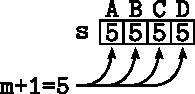
\includegraphics[scale=0.9]{../fig/quicksearch-1.pdf} 
		\end{figure}
	\item \textbf{Anpassen des Shiftarrays für vorkommende Zeichen 
		im Pattern} \\
		Das Pattern \verb!p! wird durchlaufen mit Index \verb!i!
		und \verb!m!$-$\verb!i! in das zutreffende Element vom
		Shiftarray eingetragen. Die kleine Zahl überwiegt!
		\begin{figure}[h!]
			\centering
			\hfill{} \hfill{}
			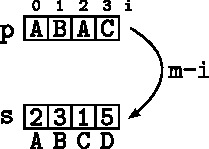
\includegraphics[scale=0.9]{../fig/quicksearch-2.pdf}
			\hfill{}
			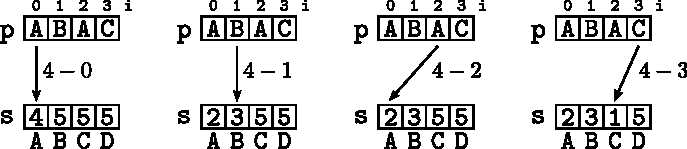
\includegraphics[scale=0.9]{../fig/quicksearch-3.pdf}
		\end{figure}
\end{enumerate}

\noindent
Nachdem das Shiftarray \verb!s! initialisert worden ist, kann mit der
Suche begonnen werden. Hierzu nimmt man das erste Zeichen des Patterns
\verb!p! und verlgeicht mit dem ersten Zeichen der Zeichenfolge \verb!a!.
Stimmt das Zeichen aus Pattern und Zeichenfolge überein, dann vergleicht
man das nächste Zeichen usw. Stimmen die Zeichen nicht überein, so
muss man in der Zeichenfolge \verb!a! vorrücken und zwar um so viele 
Stellen, wie es bis zum Ende des Pattern \verb!p! noch gibt $+1$.

\begin{figure}[h!]
	\centering
	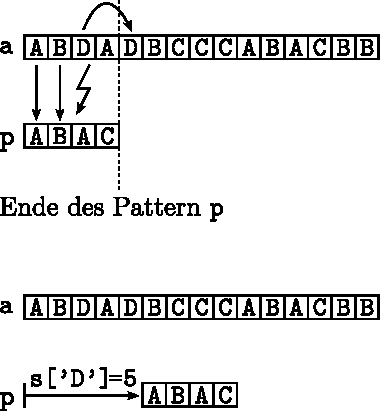
\includegraphics[scale=0.9]{../fig/quicksearch-7.pdf}
\end{figure}

\subsubsection{Implementierung}
\lstinputlisting[title=Quicksearch in Java]{quicksearch.java}



